
\begin{figure}[h]
        \centering
        \begin{subfigure}[b]{0.480\textwidth}
            \centering
            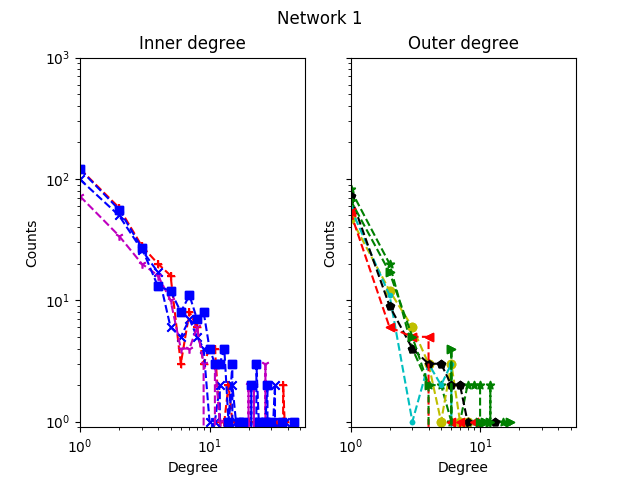
\includegraphics[width=\textwidth]{img/corpus/network1_1}
            \caption {{\small Network 1}}    
            \label{fig:mean and std of net14}
        \end{subfigure}
        \hfill
        \begin{subfigure}[b]{0.480\textwidth}  
            \centering 
            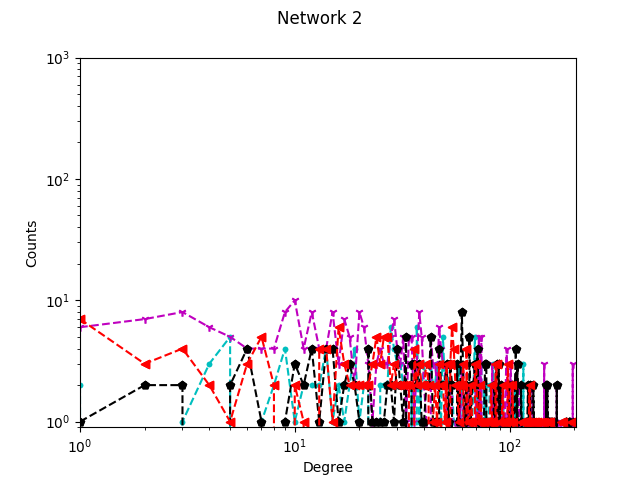
\includegraphics[width=\textwidth]{img/corpus/network2_1}
            \caption {{\small Network 2}}    
            \label{fig:mean and std of net24}
        \end{subfigure}
        \vskip\baselineskip
        \begin{subfigure}[b]{0.480\textwidth}   
            \centering 
            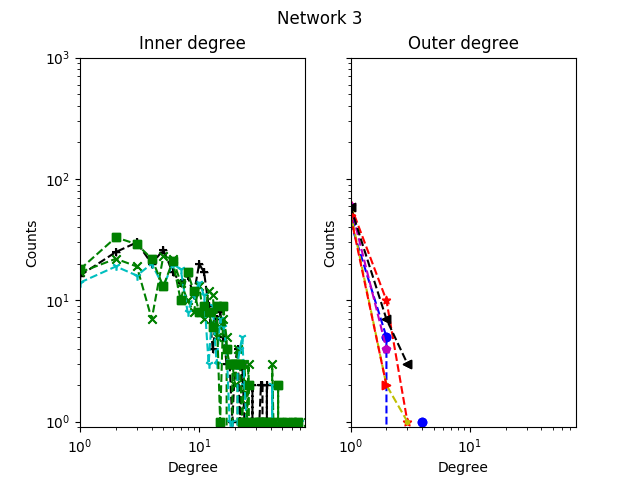
\includegraphics[width=\textwidth]{img/corpus/network3_1}
            \caption{{\small Network 3}}    
            \label{fig:mean and std of net34}
        \end{subfigure}
        \quad
        \begin{subfigure}[b]{0.480\textwidth}   
            \centering 
            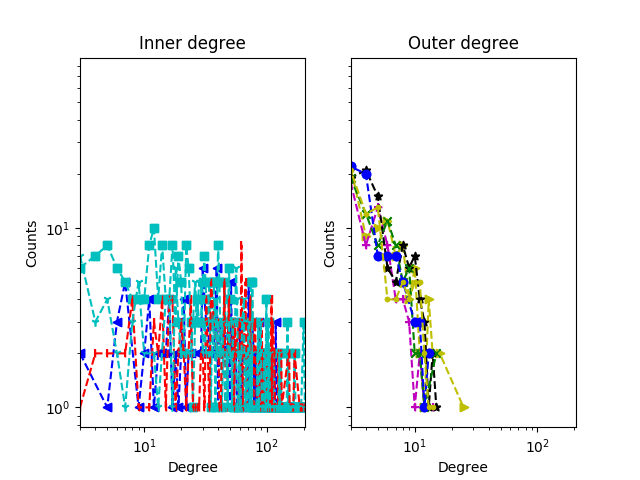
\includegraphics[width=\textwidth]{img/corpus/network4_1}
            \caption{{\small Network 4}}    
            \label{fig:mean and std of net44}
        \end{subfigure}
        \caption {Local degree distribution for the artificial networks. Inner(left) and outer(right) degree are separated.} 
	\label{fig:synt_graph_local}
\end{figure}
